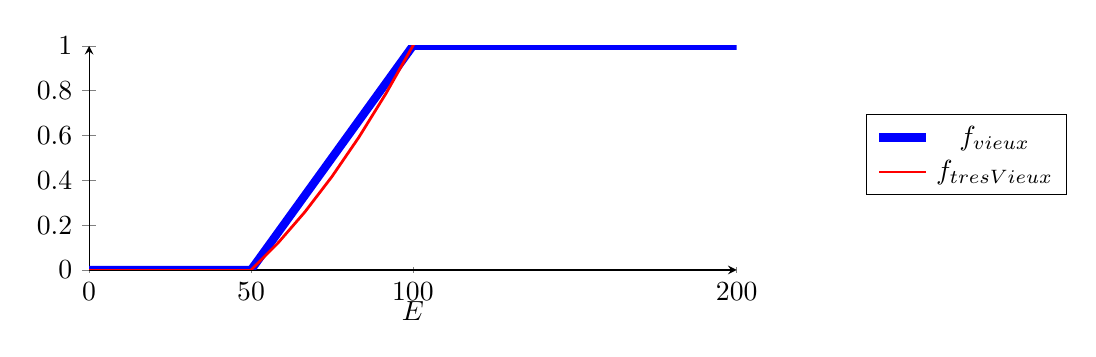
\begin{tikzpicture}
	\begin{axis}[
		xmax=200,
		ymin=0,
		ymax=1,
		xlabel={$E$},
		axis x line=bottom,
		axis y line=left,
		xscale=1.2,
		yscale=0.5,
		xtick=data,
		legend entries={$f_{vieux}$,$f_{tresVieux}$},
		legend style={at={(1,1)},anchor=south west}]
		
			\addplot+[mark=none,line width= 3] coordinates{(0,0)(50,0)(100,1)(200,1)};
			\addplot+[mark=none,line width= 1,red] coordinates{(0,0)(50,0)};
			\addplot+[domain=0:200,mark=none,line width= 1,red] {1/7500*x^2-5/15};
			
	\end{axis}	
\end{tikzpicture} 
